\subsection{Phase transitions}
We are familiar with the concept of \emph{phase transitions}, mainly from the everyday experience of the different phases of water, this concept is more general and can be applied to many systems other than the usual states of matter, such as in the study of ferromagnetic materials or even the universe in its early stages. 

In general, we have a phase transition when some thermodynamic variable exhibit a discontinuity. It is useful to label the different phase transition by which thermodynamic variable is discontinuous: mainly we distinguish \textbf{first order phase transitions}, when one of the first derivatives of the free energy is discontinuous, and \textbf{second order phase transition}, that are continuous in the first derivatives but not in the second. There can be also other kind of phase transitions, but for our purpose we just have to know that a phase transition occurs when we have a discontinuity of some thermodynamic variable.
\subsubsection{Ising model}
One of the easiest model that was first studied for phase transitions is the \emph{Ising model}: this describes a system of $N$ atoms with some "classical spin", represented by a discrete variable (that usually can be $\pm 1$). These atoms are arranged in a lattice and each pair of neighbors can interact together. 

Once the structure of the atoms is defined, the interactions are determined by the Hamiltonian of the system
\begin{equation}
    \label{Ising_Hamiltonian}
    \mathcal{H}(\sigma)=\sum_{i,j \\ \text{ neighbors}} (-J_{ij})\sigma_i\sigma_j-H\sum_i \sigma_i,
\end{equation}
where $\sigma_i=\pm 1$ is the spin of the $i$ atom, $J_{ij}=J_{ji}$ is the interaction constant between atom $i$ and $j$ and $H$ is an external field that can influence the system. From this Hamiltonian, it is clear that if $J_{ij}>0$ aligned spins will generate lower energy states (all terms of the first sum are negative), in this case the model have a \textbf{ferromagnetic} behavior, while if $J_{ij}<0$ aligned spins states will have the highest energies, in this case we have an \textbf{antiferromagnetic} behavior.

Without doing any calculation we can catch the main features of the system just by having in mind that equilibrium is reached (in the canonical ensemble since the number of atom is fixed) when the free energy 
\begin{equation*}
    F=E-TS=-\frac{1}{\beta}\log Z_{N},\qquad \text{with }Z_{N}=\sum_{\{\sigma_i\}}\exp\{-\beta\mathcal{H} (\sigma)\},
\end{equation*}
is at a minimum point. Considering a zero external field ($H=0$) and $J_{ij}>0\ \forall i,j$:
\begin{itemize}
    \item at \textbf{low temperatures} the main contribution to $F$ comes from $E$, which have a minimum when all spins are aligned, thus at low temperatures we expect all the spins to align;
    \item at \textbf{high temperatures} the contribution given by $TS$ is not negligible anymore, furthermore we cannot expect to have low energies at high temperatures, therefore the only way to minimize the free energy is by maximizing entropy, this is achieved by having all spins randomly aligned.
\end{itemize}
We can measure the overall alignment of the spins by introducing the \textbf{magnetization} $m=\frac{\sum_i\langle \sigma_i\rangle}{N} $: at low $T$ we expect to have $m\neq 0$ while at high $T$ we expect $m=0$.
\subsubsection{Mean field approximation}
To achieve a better description of the system, we can employ the \emph{mean field approximation}: this approximation becomes exact in higher dimension but also exact solutions for the lower ones can be found. We will now study this approximation assuming that $J_{ij}=J\ \forall i,j$.

Mean field approximation is obtained by neglecting fluctuation of each spin from the magnetization of the system (their mean), this can be done linearizing the interaction:
\begin{align*}
    \sigma_i\sigma_j &= [m+(\sigma_i-m)][m+(\sigma_j-m)]\\&=m^2+m(\sigma_i-m)+m(\sigma_j-m)+\underbrace{(\sigma_i-m)(\sigma_j-m)}_{negligible}\\&\simeq m^2+m(\sigma_i-m)+m(\sigma_j-m)=-m^2+m(\sigma_i+\sigma_j).
\end{align*} 
In this way the Hamiltonian now reads
\begin{equation*}
    \mathcal{H}_{MF}(\sigma)=-J\sum_{i,j \\\text{ neighbors}} [-m^2+m(\sigma_i+\sigma_j)]-H\sum_i \sigma_i,
\end{equation*}
having linearized the interaction term, we can express it as a field interaction term (as the external one), to do so we should first define the number of neighbors of each atom $z$, in this way we can run the first summation over the appearing index of each term and then, for each one, on its neighbors (having linear terms this sum is just a multiplication by $\frac{z}{2}$, where the over two factors is needed to avoid double counting the interactions)
\begin{align}
    \nonumber 
    \mathcal{H}_{MF}(\sigma)&=-J\frac{z}{2}[-Nm^2+2m\sum_{i}\sigma_i]-H\sum_i \sigma_i\\
    \label{mean_field_hamiltonian}&=\frac{JNm^2z}{2}-(Jzm+H)\sum_{i}\sigma_i.
\end{align}
As already mentioned, now the interactions appear as a sort of external field generated by the overall magnetization of the system: note that this field depends also on the geometrical proprieties of the system through $z$.

The \eqref{mean_field_hamiltonian} now allows us to evaluate the canonical partition function of the system
\begin{align*}
    Z_{N}^{MF}&=\sum_{\{\sigma_i\}}\exp\{-\beta\mathcal{H}_{MF} (\sigma)\}\\&=e^{-\beta\frac{JNm^2z}{2}}\sum_{\{\sigma_i\}}e^{\beta(Jzm+H)\sum_i \sigma_i}=e^{-\beta\frac{JNm^2z}{2}}\sum_{\{\sigma_i\}}\prod_{i}e^{\beta(Jzm+H)\sigma_i}\\&=e^{-\beta\frac{JNm^2z}{2}}\prod_{i}\sum_{\sigma_i=\pm1}e^{\beta(Jzm+H)\sigma_i}=e^{-\beta\frac{JNm^2z}{2}}(2\cosh[\beta(Jzm+H)])^N.
\end{align*}
From the partition function we can evaluate the free energy
\begin{equation}
    \label{mf_free_energy}
    F_{MF}=-\frac{1}{\beta}\log Z_{N}^{MF}=\frac{Jm^2z}{2}N-\frac{N}{\beta}\log\{2\cosh[\beta(Jzm+H)]\},
\end{equation}
this let us understand the behavior (in Fig. \ref{Fig:free energy} we can see how $F$ varies at different temperatures) that we previously just sketched.\newpage Supposing the absence of the external field $H=0$:
\begin{itemize}
    \item at high temperatures ($\beta \rightarrow0$) we can Taylor expand the logarithm at the second order to get the following approximation of the free energy 
    \begin{equation*}
        \frac{Jm^2z}{2}N-\frac{N}{\beta} \frac{1}{\cosh^2(0)}  (\beta Jzm)^2=JzN\bigg(\frac{1}{2}-\beta Jz\bigg)m^2,
    \end{equation*}
    which is a parabola with a minimum in $m=0$;
    \item at low temperatures ($\beta \rightarrow\infty$) we can approximate $2\cosh(x)\simeq e^{|x|}$, and thus the free energy \eqref{mf_free_energy} goes as 
    \begin{equation*}
        \frac{Jm^2z}{2}N-\frac{N}{\beta}|\beta Jzm|= NJz|m|\bigg(\frac{|m|}{2}-1\bigg)
    \end{equation*}
    which is a parabola mirrored along the $y$ axis, with minima in $m=\pm1$, for which all spins are aligned.
\end{itemize}
\begin{figure}[h]
    \centering
    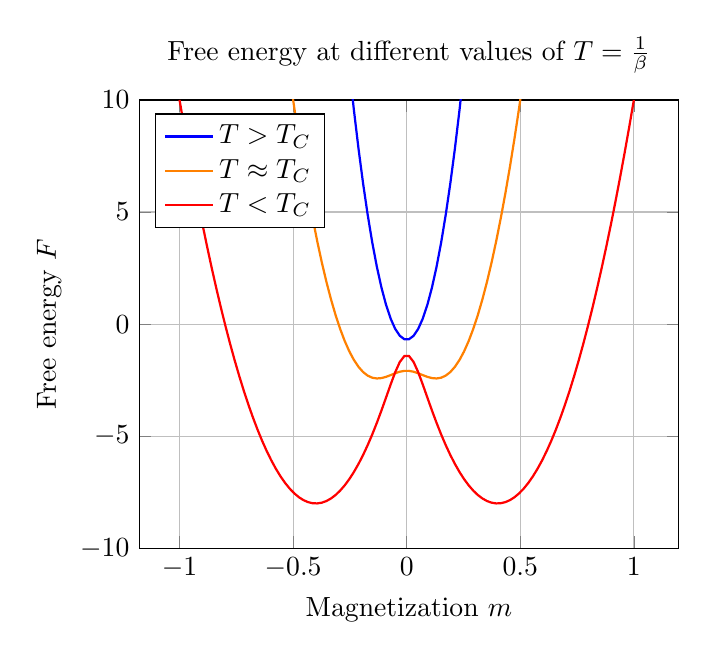
\begin{tikzpicture}
        \begin{axis}[
            ylabel=Free energy $ F$,
            xlabel=Magnetization $m$,
            ymin=-10,
            ymax=10,
            legend pos=north west,
            grid=major,
            title={Free energy at different values of $T=\frac{1}{\beta}$}
        ]
        \addplot[domain=-1:1, samples=100, blue, thick] {x^2*200 - 1 * ln(2*cosh(x/2*10))};
        \addlegendentry{$T> T_C$}
        \addplot[domain=-1:1, samples=100, orange, thick] {x^2*100 - 3 * ln(2*cosh(x*10))};
        \addlegendentry{$T \approx T_C$}
        \addplot[domain=-1:1, samples=100, red, thick] {x^2/2*100 - 2 * ln(2*cosh(x*20))};
        \addlegendentry{$T < T_C$}
        \end{axis}
        \end{tikzpicture}
    \label{Fig:free energy}
    \caption{Free energy of the system at different temperatures with a zero external field: here it is shown how $F$ goes from having a minimum in $m=0$ to having two distinct minima for $m\neq0$.}
\end{figure}
Known this, we can study these minima and so determine the magnetization of the system
\begin{equation}
    0=\frac{\partial F_{MS}}{\partial m}=Jz\{m-\tanh[\beta(Jmz+H)]\}, \quad \Rightarrow\quad m=\tanh[\beta(Jmz+H)],\label{mean_field_magnetization_equation}
\end{equation}
which is the solution of this transcendental equation. Unfortunately, being transcendental, this equation cannot be exactly solved, but we can determine when we transition from the single solution (the previous minimum in $m=0$) to multiple solutions (the two minima in $m=\pm1$ for example). Examining the graph (Fig. \ref{Fig:Soluzione m}) of the two functions equated by \eqref{mean_field_magnetization_equation} we can observe that, assuming no external field:
\begin{figure}[h]
    \centering
    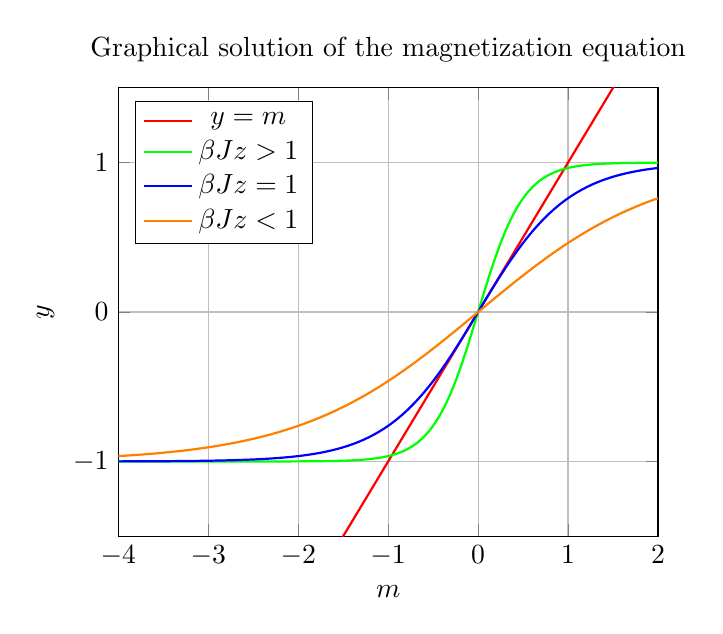
\begin{tikzpicture}
        \begin{axis}[
            xlabel=$m$,
            ylabel=$y$,
            ymin=-1.5,
            ymax=1.5,
            xmin=-4,
            xmax=2,
            legend pos=north west,
            grid=major,
            title={Graphical solution of the magnetization equation}
        ]
        \addplot[domain=-4:2, samples=2, red, thick] {x};
        \addlegendentry{$y = m$}
        \addplot[domain=-4:2, samples=100, green, thick] {tanh(2*x)};
        \addlegendentry{$\beta Jz>1$}
        \addplot[domain=-4:2, samples=100, blue, thick] {tanh(x)};
        \addlegendentry{$\beta Jz =1$}
        \addplot[domain=-4:2, samples=100, orange, thick] {tanh(0.5*x)};
        \addlegendentry{$\beta Jz<1$}
        \end{axis}
        \end{tikzpicture}
    \label{Fig:Soluzione m}
    \caption{Resolution of the implicit equation defining the magnetization for 3 different temperatures.}
\end{figure}
\begin{itemize}
    \item if $\frac{\partial}{\partial m}\tanh(\beta Jmz)\big|_{m=0}=\beta Jz\leq1$ then we have only one point of intersection in $m=0$;
    \item if $\frac{\partial}{\partial m}\tanh(\beta Jmz)\big|_{m=0}=\beta Jz>1$ then we have 3 intersections between the two functions.
\end{itemize}
This shows us that there is a temperature, that we call \textbf{critical temperature} $T_c=Jz$, before which the magnetization is exactly zero, and then it transitions to being non-zero, since a further inspection of the above stationary points will show that for $T>T_c$ the point $m=0$ becomes a maximum.

Even though we showed that the system spontaneously transitions between a magnetized state to a zero magnetization state, we haven't showed that this is a phase transition, we will now look for discontinuity in the thermodynamic variables. Consider the magnetic susceptibility
\begin{equation*}
    \chi=\frac{\partial m}{\partial H}=\frac{\partial }{\partial H}\tanh(\beta(Jzm+H))=\beta\frac{1+Jz\frac{\partial m}{\partial H}}{\cosh^2[\beta(Jzm+H)]},
\end{equation*}
once solved this equation can be evaluated at the critical temperature in absence of external fields to get
\begin{equation}
    \chi(H=0,T=JZ)=\frac{\beta}{\cosh^2(\beta(Jzm+H))-JZ\beta}\bigg|_{H=0,T=JZ}\rightarrow\infty.
\end{equation}
We should also mention that the specific heat at constant volume diverges at the critical temperature, however the mean field approximation cannot show this discontinuity.
\subsubsection{Spontaneous symmetry breaking}
We should highlight a peculiar propriety of the Ising model. Notice that the Hamiltonian \eqref{Ising_Hamiltonian}, in absence of the external field $H$, is invariant under the discrete symmetry $\mathbb{Z}_2$, defined by $\sigma_i\rightarrow\sigma_i'=-\sigma_i$. Note that the interaction with the external magnetic field explicitly breaks this symmetry: we could interpret $\mathbb{Z}_2$ as a consequence of isotropy of space, in this way the external field defines a preferred direction breaking the isotropy of space.

From this symmetry, we could argue that at equilibrium we should be in a $\mathbb{Z}_2$ invariant state, a state for which $m=0$. As we saw this is not true at every temperature: above the critical temperature the magnetization is zero, and thus we respect $\mathbb{Z}_2$ symmetry, while below the critical temperature the magnetization is non-zero, breaking the symmetry. Note that the Hamiltonian possesses the $\mathbb{Z}_2$ symmetry in both cases, therefore there is none explicit breaking of the symmetry, on the contrary with what happened with the external field. Even the mean field interaction term of \eqref{mean_field_hamiltonian} does not break the symmetry, since if $\sigma_i\rightarrow\sigma_i'=-\sigma_i$ also $m\rightarrow m'=-m$ (in the Hamiltonian appears their product). In this case we have a \textbf{spontaneous breaking of the symmetry}.

What actually happens here is that the "\emph{ground state}" breaks the symmetry, since as we saw a single minimum splits into two different minima, then the system could hypothetically remain in a stationary state which preserve the symmetry (in this case $m=0$) but that would be an unstable state. At this point thermal fluctuations are enough to move the system to a minimum breaking the symmetry.

This kind of behavior, not only is interesting to be studied per se, but it revealed to be key into the development of many deep mechanisms of nature, first over all the Higgs mechanism that gives mass for example to gauge bosons in the standard model. 

\subsubsection{Exact solutions}
We employed the mean field approximation just to illustrate the general behavior that we should expect from the system, however if we want to study this system some exact results should be used too. 

Mean field approximation fails for a lattice of dimension 1, since it would predict a $T_c=2J$ while the exact solution predicts that there is no spontaneous symmetry breaking in this case. For higher dimension than 4 the approximation become suitable while at lower the exact results can differ, as happens for dimension 1. In dimension 2, some non-trivial exact solutions can be found: we present the exact critical temperature for some simple topology of the lattice, these results can be found in \cite{ExactIsing}:
\begin{align}
    &\text{Square lattice: } &T_c^S&=\frac{2}{\log(1+\sqrt{2})}J &\simeq 2.26929 J,&&\\
    &\text{Triangular lattice: } &T_c^T&=\frac{2}{\log(\sqrt{3})}J &\simeq 3.64096 J,&&\\
    &\text{Hexagonal lattice: } &T_c^H&=\frac{2}{\log(2+\sqrt{3})}J &\simeq 1.51865 J.&&
\end{align}
These results can be compared to the mean field ones: $T_c^{S}=4J,\ T_c^{T}=6J$ and $T_c^H=3J$. In this way we can see that mean field approximations should be considered as an estimate of an upper bound of the critical temperatures.
